\documentclass[british,a4paper, 12pt]{article}
\usepackage[hidelinks]{hyperref}
\usepackage{babel}
\usepackage{csquotes}
\usepackage[backend=biber,style=apa]{biblatex}
\addbibresource{ethics-essay.bib}
\usepackage{graphicx}

\DeclareLanguageMapping{british}{british-apa}

\title{Ethical Considerations for the $21^{st}$ Century in Bioinformatics and Medical Practice}
\author{Michael J. Jones \\
  MSc Bioinformatics \& Computational Genomics \\
  Queen's University Belfast}

\date{\today}
\begin{document}
\maketitle
  
\section{Introduction}
In 2006, Professor Herman Tavani wrote that both Information Technology and
genetics will play a critical role in $21^{st}$ century healthcare. As part of
this rapid development, Bioinformatics as a field is exemplary of how
Information Technology is required to collate, analyse and distribute genetic
data \parencite{tavani2006ethics}[Chp.~17].

The abundance of data available in the form of genetic and image data raises
concerns for privacy of individuals. The fact that Informatics has come to
play such a critical role in biomedical research poses problems ethically.
Fields such as Bioethics and Computational ethics have had years to develop
independently.

Hongladarom argues that Bioinformatics poses a whole new paradigm of ethics in
terms of data protection. While data protection measures are in place for the
safe keeping of credit card numbers in order to protect the identity of an
individual, storing a persons full genome or exome sequence adds an additional
challenge in that your genetic sequence is inherently and indelibly part of
your identity \parencite{hongladarom2006ethics}.
v
Add to this, in clinical trials it becomes favourable among researchers to 
store medical records in a digital format which provide so many benefits (e.g. 
such that data need only be entered once into a computer system for statistical 
analysis) \parencite{parizel2011keep} that justifying using other methods comes to seem
counter-productive even though the ease with which this data can be disseminated among
different interest groups becomes far easier.

This article will expand on some of the ethical challenges that come with
Bioimaging and Bioinformatics with particular attention given to the storing
of data and tissue in Biobanks, followed by a discussion of the ethics of
image manipulation in a scientific context.

\section{Biobanks}
An important element for successful scientific enquire in the field of
Bioinformatics is the availability of large data sources for processing. The
term `biobank` is a confounding term resulting from a range of different
interpretations, be they the storage of tissue samples, DNA sequence data or
medical images.

An early and comprehensive example of a Biobank took blood samples from the
many Icelandic citizens including data from their medical records. deCODE
genetics is a private biotechnology company from Delaware that was allowed to
gain access to these records following a law passed in the Icelandic parliament
in 1998 \parencite{chadwick1999icelandic}.

These biobanks become an increasingly important part of medical research and 
it can be argued they will become even more relevant with a move towards 
personalised medicine \parencite{watson2010integrating}. An example of this
includes the identification of imatinib for targeting chronic myeloid leukaemia 
in particular subpopulations \parencite{cohen2002approval} as well as in the
application of herceptin in certain breast cancers \parencite{lemieux2009role}.

A number of ethical issues have been raised 
following the decision of the Icelandic parliament. These issues will be 
discussed below.

\subsection{Data protection}
A large proponent of the criticism of the deCODE genetics project is the issue
of informed consent with regard to gaining access to individuals private
medical data.

The Icelandic Government in the case of deCODE project decided that informed 
consent would not be required to collate the medical records and blood samples 
of its citizens because it would be anonymised \parencite{chadwick1999icelandic}.

\emph{The European Directive on the Protection of Personal Data}, officially 
termed 95/46/EC, is a directive issued by the European Union (EU) from 1995 which 
addresses the issue of processing of personal data. Article 8 of this directive 
prohibits the processing of certain types of personal data such as that which 
can reveal the racial or ethnic origin of a person as well as prohibiting the 
processing of data concerning a person's health \parencite{directive199595}.

Exhemptions stated in this directive include seeking the ``explicit consent'' 
of individuals unless a member state of the European Union has laws to override 
this. In this regard, deCODE genetics should, according to the EU directive 
should have regardless of the Icelandic government's laws, seeked the consent of 
the Icelandic citizens \parencite{carey2009data}.

Knowing that this is in fact a legal as well as an ethical issue, Research Ethics 
Committees (RECs) and Institution Review Boards (IRBs) have an important role in 
ensuring that the consent of patients is sought for all material stored in a 
biobank \parencite{watson2010integrating}.

In light of data protection laws that govern all personal data within the European Union,
biobanks now require far more stringent measures to ensure that the interests of individuals
putting their data into biobanks are protected. Including requiring the explicit signing of
consent forms by patients detailing the ways in which their tissue and data samples could
be used in the future.

Observing the increasing length and complexity of these consent forms,
\citeauthor*{beskow2010simplifyinog} conducted a study in which they drafted a sample consent form
for a biorepository. They asked cohorts of patients, researchers and IRB staff to underline
sentences within the consent form using a tablet computer. The results of these findings were
then loaded into SAS (\url{http://www.sas.com}) software to analyse the frequencies and the nature
of sentences highlighted by the different interest groups \parencite{beskow2010simplifyinog}.

Reassuringly, the number of lines underlined by IRB staff, researchers and patients decreased in
each respective group, implying that of everyone, the patients displayed the lowest concern for
their personal data. Furthermore, if IRB staff preferred to include more of the lines in the
consent form than researchers which could mean that researchers display less concern with the
informing a patient of how their data will be used. Conversely, this might also imply that IRB
representatives practised greater stringency to justify their positions. We also know that
researchers are, in practice, looking to maximise the number of participants in their studies
whereas IRB staff are tasked with protecting the rights of patients.

\section{Electronic Medical Records}
The Electronic Frontier Foundation (EFF) identifies an electronic medical record as
the digital record of information that is generated in a medical institution which may
include laboratory results, information about immunisation of a patient,
details of prescription and even the demographics of a patient
\cite{effemrdefinition}.

As discussed earlier in this article, we presented the data protection issues of storing
patient data in biobanks. While the purpose of the biobank is to aid research, Electronic
Medical Records (EMR) are meant to ease medical practice. As with other digitised media,
EMR are presented as a panacea for a number of problems that exist with paper-based
systems.

With regards to primary care, the United Kingdom (UK) has observed a very high percentage
of medical practices adopting EMR systems with close to 100\% of practices using some sort
of EMR system as compared to the United States (US) where adoption has been relatively poor.
The reason for the high adoption rates in the United Kingdom, where General Practitioners (GPs)
surgeries have paid for these systems themselves, is due to the convenience of e-prescribing
offered by these systems which GPs felt increased the efficiency and lowered the risk of
errors caused by illegible handwritten prescriptions \cite{schade2006prescribing}.

% Having discussed other issues
In medical practice, EMR system adoption is motivated by convenience, saving of time and 
minimising of errors. While these are justifiable reasons for using EMR, the convenience 
afforded by these systems may come at the risk of jeapordising the confidentiality of 
patient data. Evidence of this trend is seen in Korea where EMR systems are already widely 
used in hospitals with a movement towards using mobile devices such as smartphones to 
access these data \parencite{yeo2012pitfalls}.

\citeauthor*{kluge2000professional} identifies 7 principles that should be adhered to
with regard the treatment of medical records. These principles,
\citeauthor*{kluge2000professional} write, should be independent of national or ethnic
values and that we cannot depend on legal frameworks to impose such principles due to
the fact that laws are determined for reasons other than the ethical which might lead to
conflicting outcomes \parencite*{kluge2000professional}.

One issue raised in the above article involves the ``Principle of security'' which
addresses the issue of protecting an individuals medical data against modification or
disclosure to other parties. The illegitimate access of medical records,
as evidenced by one doctor in 2009 who accessed the medical records of Alex Salmond,
First Minister of Scotland the then UK Prime Minister, Gordon Brown
\parencite{dailyrecord2010doctor} is a concern which makes real the fact that, EMR
systems should not be accessible to all medical staff without the consent of a patient.

Particular care should be taken to implement EHR so that their benefits are not in the 
name of convenience and economic reasons. Attempts to rush in the advent of EHR in the 
United States have been made by members of its Congress by motivating clinical 
practitioners to use EHR  by allocating each a \$44\,000 to encourage ``meaningful use'' 
\parencite{jha2010meaningful}.

\section{Bioimaging}
In both the fields of research and soon the field of clinical pathology, imaging is becoming 
increasingly important. In the medical setting, some institutions such as Pathology Department 
in the University Medical Center of Utrecht perform digital slide scanning of all pathology 
slides for archiving and education purposes. They have been doing this since 2007
\parencite{stathonikos2013going}.

Data protection measures that affect medical and personal data should also be 
applied to medical imaging data, knowing that these images are themselves a form 
of personal data \parencite{duquenoy2008considering}. The ethical issues in terms of storage
and dissemination of medical images should therefore be treated with the same
sensitivity as with other medical data be that in biobanks or as part of a person's
medical record.

One other controversial issue of the use of digital imagery in both fields of research and 
clinical practice is the ability to digitally enhance images such that, to the naked eye, they 
can tell a different story. \citeauthor*{cutrone2001true} observed in the early 2000s the ease 
with which image manipulation software could be obtained for use on personal computers  (such as 
Photoshop and Paintshop Pro) leading to a situation where the ability to legitimately and 
fraudulently ``touch up'' images could be harnessed by anyone \parencite{cutrone2001true}. (See
figure \ref{fig:cutroneimage}.)

In fact, in 2006, an editorial posted in Nature stated that the Journal of Cell Biology's
managing (BCJ) director stating that in their experience, 25\% of submitted articles had figures that
had to be remade and, in 1\% of those cases, fradulent changes were observed. Somewhat amusingly,
yet also soberingly, it was also found that at least two of these articles were then published
in other publications \parencite{cromey2009digital}.

Guidelines exist regarding the ethical and unethical manipulation of digital images in journalism as
stated in guidelines published by the National Press Photographers Association (which are
published on their website \parencite{national2012ethics}. Such guidelines have been available to
journalists regarding the legitimate and illegitimate digital manipulation of images have been
available since the early 1990s \parencite{cromey2010avoiding}.

To address this problem, in 2001, \citeauthor*{cromey2001digital} drafted a number of guidelines for
the editing of digital images in an ethical way \parencite{cromey2001digital}. These guidelines,
in summary, can be seen in Figure \ref{fig:ethicalguidelines}.

\begin{figure}

\begin{itemize}
\item Images are data that can be inappropriately manipulated
\item Always do image manipulations on a copy of an unprocessed image
\item Simpler manipulations to an image are more likely to be acceptable
\item Cropping an image is acceptable in most cases
\item When comparing images, both images should be taken under the same conditions and exposed to the same manipulations
\item Usually, manipulating portions of an image instead of applying a transformation to a whole image is illegitimate
\item Using software filters to enhance the quality of biological images is not advisable
\item Cloning and copying of artefacts into another image is extremely questionable
\item Know the limitations of the equipment used to record images
\item Avoid ``lossy'' compression of images
\item Knowing the ratio of pixels to centimetres is important when analysing images
\item Changing the size of an image in pixels can cause data loss
\end{itemize}

\caption{An abbreviation of the guidelines presented by \parencite{cromey2001digital}.}
\label{fig:ethicalguidelines}
\end{figure}


In response to issues highlighted by Cromey and the findings of the BCJ, respectable
journals have responded by posting guidelines online, albeit, as in the case of Nature,
these guidelines are relatively vague and brief \parencite{natureimg}. While it may be a
cause concern, it is likely that there is still much debate to be had with regard to image
editing in journal publications.

\begin{figure}
\caption{An example of retouching an image of a child to hide an hemangioma of the left arm.}
\label{fig:cutroneimage}
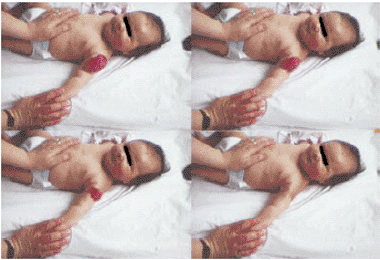
\includegraphics[natheight=\textheight,natwidth=\textwidth]{images/cutrone2001fig.png}

\end{figure}

\section{Conclusion}

What remains to be seen is how the ethical challenges presented in our informatics driven
world of medicine and research are addressed in different states knowing that, just as there
are a variety of laws that govern the nations of the world, so also values and traditions will
vary \cite{kluge2000professional}.


\printbibliography

\end{document}

%%  LocalWords:  EHR
